Ramsey Theory follows an interesting theorem stating that for any positive integers $r$ and $s$, there is a least positive integer $R(r,s)$ such that every blue-red edge coloring of $K_{R(r,s)}$ has a blue clique with $r$ vertices or a red clique with $s$ vertices. One extensively studied problem is calculating such $R(r,s)$ which proves to be very hard, even for very small values of $r$ and $s$. 

The relation of any blue-red edge coloring of a graph $G$ having either a blue clique of size $r$ or a red clique of size $s$ is denoted by $G\rightarrow(r,s)^e$. Similarly defined, if every edge coloring of $G$ has either a blue copy of $H$ or a red copy of $F$, then $G\rightarrow(H,F)^e$. In a special case, where $H$ is isomorphic to $F$, the \textit{Ramsey Arrowing} is denoted by $G\rightarrow(H)^e$. Another set of problems arise when considering the online version of the problem.

\subsection*{On-line Ramsey Theory\cite{1}}

The word ``online" means that, when checking if $G\rightarrow(H)^e$, the edge coloring of $G$ takes place before the entirety of $G$ is known. The typical way, introduced by \textit{Online Ramsey Theory}\cite{1}, to present the online version of the problem is through a combinatorial game between painter and builder:

\begin{adjustwidth}{2em}{2em}
	\noindent\underline{Online Ramsey Game:}
	Take an unbounded set of vertices with no edges and a target graph $H$. Builder selects two disconnected vertices and adds an edge between them. Following, Painter colors the introduced edge. If a monochromatic copy of $H$ is ever created, then the Builder wins. Painter wins if it provides a strategy to avoid $H$ indefinitely.
\end{adjustwidth}

If the builder provides the edges of $G$, and $G\rightarrow(H)^e$, then the builder wins, because there is no possible way to paint the edges of $G$ while avoiding $H$, as defined above. However, it is not true that if the painter cannot prevent $H$, when given edges of $G$, then $G\rightarrow(H)^e$. The mismatch comes from an additional challenge the painter faces on the online version. The added challenge of the online version comes from the lack of information when the Painter takes its decisions.

Consider now a slightly different version. In this version, the builder can only create graphs belonging to a class of \mbox{graphs $\mathcal{G}$.} Considering that $H \in \mathcal{G}$, $H$ is called unavoidable if the builder can force the painter to create a monochromatic copy of $H$, and called avoidable otherwise. If every graph of a class is unavoidable, then the class is called self-unavoidable.

Together with the formulation of these problems the authors show\cite{1} that the class of forests is self-unavoidable, also mentioned in the second section. For this proof, check the visualization featured in the application or in the original paper. An important comment on this self-unavoidability and the difference between the online and offline version of the problem is that forests are clearly avoidable in the offline version.

On the offline version, in fact, it is possible to avoid $P_4$ by following a simple strategy. Elect roots for all the trees in the forest. Color blue all the edges with odd distance to the root and red those with even distance. This strategy does not work in the online version because the distances to a root are not known at the time they are created by the builder.

When concluding their paper, the authors conjecture that the class of outerplanar graphs is exactly the class of unavoidable graphs when playing with $\mathcal{G}$ as the planar graphs.

\subsection*{Online Ramsey Theory for Planar Graphs\cite{3}}

Ten years later, Šárka Petříčková\cite{3}, proved the conjecture wrong. She showed that the builder can force all outerplanar graphs, but can also force some graphs that are not outerplanar. She proved that all outerplanar graphs are unavoidable, but, then, showed a class of graphs, that is not outerplanar, but that is unavoidable when playing on the planar graphs.

Although the proofs contain too many details to be adapted here, it is worth bringing counter examples of the conjecture. First she shows that even cycles are unavoidable. Then, she shows a strategy, based on structures consisting of even cycles, and adds edges and vertices to the graph in a way that the target graph is reached. The class of non-outerplanar graphs used by her is the class of $\theta_{i,j,k}$ with $i, j$ and $k$ even. A graph denoted by $\theta_{i,j,k}$ is composed of three internally disjoint paths of lengths $i,j$ and $k$. The graphs $\theta_{2,2,2}$ and $\theta_{2,2,4}$:

\begin{center}
	\begin{minipage}{0.55\linewidth}
		\hspace{0.5cm}
	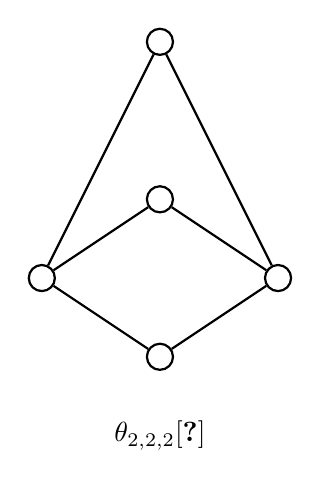
\begin{tikzpicture}[node distance={15mm}, thick, main/.style = {draw, circle}] 
		\node (title) at (1.5, -2) {$\theta_{2,2,2}$\cite{6}};
		\node[main] (1) at(0, 0) {};
		\node[main] (2) at(1.5,1) {}; 
		\node[main] (3) at (1.5, 3) {};
		\node[main] (5) at (3, 0) {}; 
		\node[main] (6) at(1.5,-1) {};
		\draw (1) -- (2);
		\draw (1) -- (3);
		\draw (1) -- (6);
		\draw (2) -- (5);
		\draw (6) -- (5);
		\draw (3) -- (5);
	\end{tikzpicture}
	\end{minipage}
	\begin{minipage}{0.35\linewidth}
	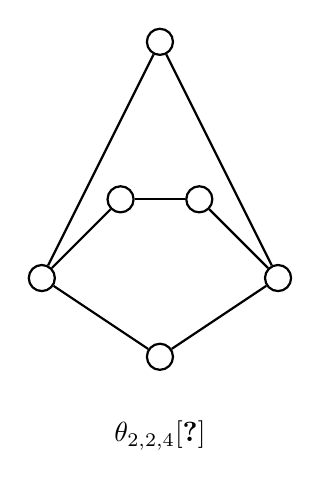
\begin{tikzpicture}[node distance={15mm}, thick, main/.style = {draw, circle}] 
		\node (title) at (1.5, -2) {$\theta_{2,2,4}$\cite{3}};
		\node[main] (1) at(0, 0) {};
		\node[main] (2) at(1,1) {}; 
		\node[main] (3) at (1.5, 3) {};
		\node[main] (4) at (2, 1) {}; 
		\node[main] (5) at (3, 0) {}; 
		\node[main] (6) at(1.5,-1) {};
		\draw (1) -- (2);
		\draw (1) -- (3);
		\draw (2) -- (4);
		\draw (1) -- (6);
		\draw (6) -- (5);
		\draw (3) -- (5);
		\draw (4) -- (5);
	\end{tikzpicture}
\end{minipage}
\end{center}

Are clearly not outerplanar, however it is possible for the builder to force a monochromatic copy of it on the class of planar graphs. Starting from a base structure composed of even-length cycles, showed in gray, the builder just have to build the edges of the graphs below, in black, extracted from Petříčková's work. 

\begin{center}
	\begin{minipage}{0.4\linewidth}
	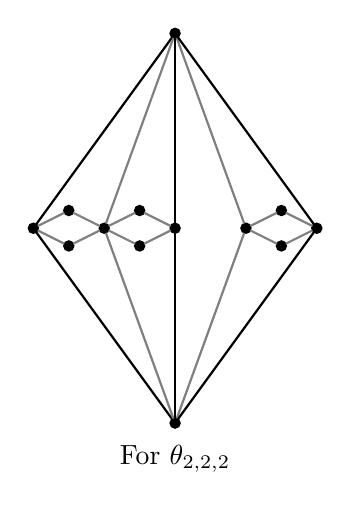
\begin{tikzpicture}[thick, main/.style = {draw, circle, fill=black,scale=0.35}, scale=0.45]
		\node (title) at (4, -6.5) {For $\theta_{2,2,2}$};
		\node[main] (1) at(0, 0) {};
		\node[main] (2) at(1,0.5) {}; 
		\node[main] (3) at (1,-0.5) {};
		\node[main] (4) at (2, 0) {}; 
		\node[main] (6) at(3,0.5) {};	
		\node[main] (7) at(3,-0.5) {};
		\node[main] (8) at(4,0) {};
		\node[main] (9) at(4,-5.5) {};
		\node[main] (10) at(4,5.5) {}; 
		\node[main] (11) at(6,0) {};
		\node[main] (12) at(7,-0.5) {};
		\node[main] (13) at(7,0.5) {};
		\node[main] (14) at(8,0) {};
		\draw[gray] (1) -- (2);
		\draw[gray] (1) -- (3);
		\draw[gray] (2) -- (4);
		\draw[gray] (3) -- (4);
		\draw[gray] (4) -- (6);
		\draw[gray] (4) -- (7);
		\draw[gray] (6) -- (8);
		\draw[gray] (7) -- (8);
		\draw (1) -- (9);
		\draw (1) -- (10);
		\draw (8) -- (9);
		\draw[gray] (9) -- (4);
		\draw[gray] (10) -- (4);
		\draw (8) -- (10);
		\draw[gray] (9) -- (11);
		\draw[gray] (10) -- (11);
		\draw[gray] (11) -- (12);
		\draw[gray] (11) -- (13);
		\draw[gray] (12) -- (14);
		\draw[gray] (13) -- (14);
		\draw (9) -- (14);
		\draw (10) -- (14);
	\end{tikzpicture}
\end{minipage}
	\begin{minipage}{0.4\linewidth}
		\includegraphics[scale=0.4]{images/theta_2_2_4.png}
		\captionof*{figure}{\hspace{0.7cm}For $\theta_{2,2,4}$}
	\end{minipage}
\end{center}

Petříčková finishes her paper by bringing to light the question whether the class of planar graphs is self-unavoidable, but conjecturing that $K_4$ is avoidable. Of course that if her conjecture is right, then the class of planar graphs is not self-unavoidable. Since 2014, however, no direct progress has been made when it comes to planar graphs, but there are some developments studying other classes.

\subsection*{Online Ramsey theory for a triangle on $F$‐free graphs\cite{3}}

In this paper there is a small shift from what has been highlighted so far. Firstly, it deals with non-planar planar graphs. Secondly, and more importantly, instead of taking a class and deciding whether it is self-unavoidable, the authors take a structure, $C_3$ and study the classes where it is unavoidable. The paper is concerned with classes of graphs where a determined structure is not a subgraph.

First, the authors show that $C_3$ is unavoidable in the class of $K_4$-minor-free graphs. A graph $G$ is a minor of another graph $H$ if, after a sequence of vertex deletions and edge removals or contractions, $G$ is obtained from $H$. This way, $K_4$-minor-free graphs are those for which $K_4$ is never obtained after a sequence of such operations. The result obtained by the authors directly extend the result proved on \textit{On-line Ramsey Theory}.

In the paper from 2004, the authors show that $C_3$ is unavoidable in the class of outerplanar graphs. This means they showed $C_3$ is unavoidable in the class of ($K_{2,3},K_4$)-minor-free graphs. This extension shows that $K_{2,3}$ is not necessary to force a triangle.

Following up, the paper presents a total of five graphs $X_1, X_2. X_3, X_4$ and $X_5$, the larger ones having six vertices. The authors claim and prove that, if a graph $F$ has no isolated vertex and is not isomorphic to $X_5$, then:
\begin{center}
Painter wins the Online Ramsey Game for $C_3$ on the class of $F$-free graphs\\$\iff$\\$F$ is isomorphic to a subgraph of either $X_1,X_2,X_3$ or $X_4$\footnote{This is specially nice because these graphs have between five and six vertices.}
\end{center}

Then, they end their paper by highlighting the only missing result for $C_3$ for such classes of graphs in Online Ramsey Games: ``Who wins the Online Ramsey game for $C_3$ on $X_5$-free graphs"?

\subsection*{One more problem}

When changing the offline problem to the online version, the Painter becomes much weaker. To balance that, restrictions are added to the Builder as well, in the form of restricting its moves to certain classes of graphs. Another option, however, would be making the painter stronger.

For this version, instead of using an unbound set of vertices, the builder has a finite number in its disposal. Additionally, consider that instead of coloring each edge in sequence, the Builder builds $k$ edges in each turn. When the Painter has to make its decisions, it has more knowledge of the overall structure. However, it is not clear whether it is meaningful or not. It actually turns out that this boost is not very meaningful\cite{7}. \textit{Ramsey games against a one-armed bandit} analyzes the problem thoroughly and, although very different from the algebraic approach presented in the other references, complements nicely the study on Online Ramsey Theory. 




